%
% k-kruemmung.tex -- Krümmungstensor, Ricci, Einstein
%
% (c) 2017 Prof Dr Andreas Müller, Hochschule Rapperswil
%
\section{Krümmung einer Fläche%
\label{skript:kruemmung:section:kruemmung}}
\rhead{Krümmung einer Fläche}

\begin{figure}
\centering
\includegraphics[width=\hsize]{chapters/3d/flach.jpg}
\caption{Beim Paralleltransport eines Vektors entlang einer Kurve in
einer Ebene dreht sich der Vektor nicht.
\label{skript:kruemmung:transportflach}}
\end{figure}

\begin{figure}
\centering
\includegraphics[width=0.65\hsize]{chapters/3d/sphere.jpg}
\caption{Drehung eines Tangentialvektors beim Transport entlang eines
Dreiecks auf der Kugeloberfläche.
Der Flächeninhalt des Dreiecks ist ein Achtel der Kugeloberfläche,
also $4\pi/8=\pi/2$, der Drehwinkel ist $\pi/2$.
\label{skript:kruemmung:transportkugel}}
\end{figure}

Transportiert man einen Vektor in der Ebene mit dem üblichen euklidischen
Koordinatensystem parallel, dann ändert seine Richtung nicht,
denn die Christoffelsymbole verschwinden alle
(Abbildung~\ref{skript:kruemmung:transportflach}).
Auf einer Kugeloberfläche sieht das ganz anders aus.
In Abbildung~\ref{skript:kruemmung:transportkugel} wird
eine Vektor tangential an den Äquator zunächst entlang 
des Äquators über einen Winkel von $90^\circ$ transportiert,
dann auf einem Längenkreis bis zum Nordpol
und wieder zurück zum Ausgangspunkt.
Es ist offensichtlich, dass sich der Vektor dabei um $90^\circ$ dreht. 
Der Unterschied rührt natürlich daher, dass die Kugeloberfläche gekrümmt
ist.
Offenbar ist die Änderung der Richtung eines Tangentialvektors beim
Paralleltransport entlang eines geschlossenen Weges ein Mass für die
Krümmung einer Fläche.

In diesem Kapitel wollen wir zeigen, wie aus dem Konzept des
Paralleltransportes ein mathematisch wohldefiniertes Mass für die
Krümmung gewonnen werden kann.
Die physikalische Bedeutung der Krümmung wie auch der Christoffelsymbole
werden wird erst im Kapitel~\ref{skript:chapter:gravitation} klären.

\section{Krümmungstensor}
%\rhead{Krümmungstensor}
Wir möchten Berechnen, wie sich ein Vektor beim Paralleltransport entlang
einer geschlossenen Kurve ändert.
In dieser Form ist das Problem sicher zu kompliziert, die Wahl
einer geschlossenen Kurve beinhaltet viel zu viele Freiheitsgrade.

\rhead{Krümmungstensor}
\begin{figure}
\centering
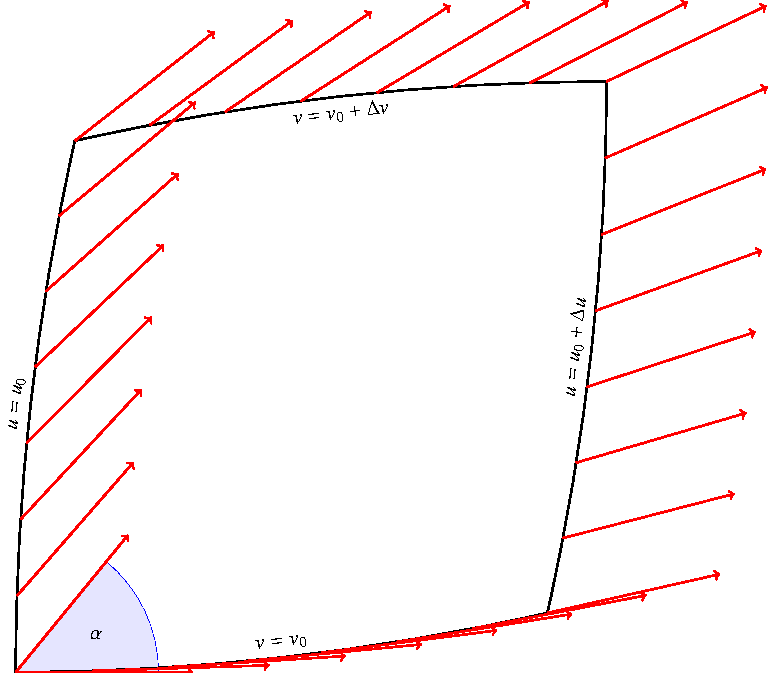
\includegraphics{chapters/tikz/riemann.pdf}
\caption{Paralleltransport eines Vektors entlang eines
Koordinaten-Parallelogramms.
\label{skript:kruemmung:parallelogramm}}
\end{figure}

Zu zwei Tangentialvektoren $u^\mu$ und $v^\mu$ und in einem Punkt
$P$ können wir immer eine
Fläche finden, die aus Geodäten besteht, die alle vom Punkt $P$ ausgehen
und dort eine Richtung haben, die eine Linearkombination der beiden
Tangentialvektoren ist.
Mit diesem Trick können wir das Problem auf eine zweidimensionale
Fläche reduzieren.
Und statt eine beliebige Kurve zuzulassen, können wir uns weiter
auf einen Polygonzug beschränken, bei dem wir den Geodäten folgen,
die als Tangentialrichtung die Richtung der beiden gegebenen
Tangentialvektoren haben.
Abbildung~\ref{skript:kruemmung:parallelogramm} zeigt, wie ein Vektor
entlang eines Koordinatenparallelogramms transport wird und sich
dabei dreht.

Wenn wir einen Vektor $A^\mu$ entlang einer solchen Kurve parallel
transportieren, dann aber die Kurve auf einen Punkt zusammenschrumpfen
lassen, dann entsteht im Grenzwert ein Vektor $y^\mu$,
der die Verschiebung des Vektors $A^\mu$ beschreibt.
Dieser Vektor muss linear von $u^\mu$, $v^\mu$ und $A^\mu$ abhängen,
wir erwarten also, dass in jedem Punkt Zahlen
$R^\alpha\mathstrut_{\mu\nu\sigma}$ geben muss, mit denen man
$y^\mu$ berechnen kann:
\[
y^\alpha = R^\alpha\mathstrut_{\mu\nu\sigma}u^\mu v^\nu A^\sigma.
\]
Da der Paralleltransport die Länge erhält, entspricht die Änderung des
Vektors einer Drehung.
$R^\alpha\mathstrut_{\mu\nu\sigma}$ codiert also das Ausmass der
Drehung des Vektors.

Zur Konstruktion des Krümmungstensors gehen wir wie folgt vor.
Im Abschnitt~\ref{skript:kruemmung:section:wegintegral} definieren
wir Integrale entlang eines Weges und über ein von einer Kurve begrenztes
Flächenstück.
In Abschnitt~\ref{skript:kruemmung:section:green} präsentieren
wir den Satz von Green, der einen Zusammenhang zwischen Weg- und
Gebietsintegral herstellt.
Der Satz von Stokes verallgemeinert dies für beliebige Kurven
im Raum in \ref{skript:kruemmung:section:stokes}.
In Abschnitt~\ref{skript:kruemmung:section:kruemmungstensor}
verwenden wir diese mathematischen Werkzeuge, um den Krümmungstensor
zu definieren.

\subsection{Wegintegral und Gebietsintegral in der Ebene%
\label{skript:kruemmung:section:wegintegral}}
In diesem Abschnitt betrachten wir Funktionen $f(x,y)$ und $g(x,y)$
in der Ebene und ein Teilgebiet $D\subset \mathbb R^2$, welches
von einer Kurve $c\colon [a,b]\to\mathbb R^2\colon t\mapsto c(t)$
berandet wird.
Die beiden Funktionen $f$ und $g$ kann man auch als ein zweidimensionales
Vektorfeld in der Ebenen $\mathbb R^2$ betrachten, jedem Punkt der
Ebene ist ein Vektor 
\[
(x,y)\mapsto \vec{v}(x,y)=\begin{pmatrix}f(x,y)\\g(x,y)\end{pmatrix}
\]
zugeordnet.

\begin{definition}
Das Wegintegral des $\vec v$ entlang der Kurve $c(t)=(x(t),y(t))$ ist
\[
\oint_c (f\,dx + g\,dy)
= 
\int_a^b f(x(t),y(t)) \dot x(t) + g(x(t),y(t)) \dot y(t)\,dt.
\]
\end{definition}

Zu dem gegebenen Gebiet $D$ kann man aber auch für jede beliebige
Funktion $h(x,y)$ das Gebietsintegral bilden.
Wir tun dies im Detail nur für Gebiete deren Rand sich durch zwei
Funktionen $y_1(x)$ und $y_2(x)$ beschreiben lassen, so dass das
Gebiet $D$ die Menge
\[
D=\{ (x,y) \,|\, y_1(x) \le y \le y_2(x), x_1\le x\le x_2\}
\]
ist.
Dann definieren wir

\begin{definition}
Das Gebietsintegral von $h(x,y)$ im Gebiet $D$ ist
\[
\int_D h(x,y)\,dx\,dy = \int_{x_1}^{x_2} \int_{y_1(x)}^{y_2(x)} h(x,y)\,dy\,dx
\]
\end{definition}

Lässt sich das Gebiet ausserdem mit zwei Funktion $x_1(y)$ und $x_2(y)$
in der Form
\[
D=\{(x,y)\,|\, x_1(y)\le x\le x_2(y), y_1\le y\le y\le y_2\}
\]
beschreiben, dann kann man das Gebietsintegral auch als
\[
\int_Dh(x,y)\,dx\,dy
=
\int_{y_1}^{y_2}\int_{x_1(y)}^{x_2(y)} h(x,y)\,dx\,dy
\]
schreiben, und die beiden Formeln stimmen überein.

\subsection{Der Satz von Green%
\label{skript:kruemmung:section:green}}
Der Satz von Green stellt einen Zusammenhang zwischen einem Wegintegral
und einem Flächenintegral her.

\begin{satz}[Green]
\label{skript:kruemmung:satz:green}
Sind $f$ und $g$ stetig differenzierbare Funktionen im Gebiet $D$, welches
von der Kurve $c$ berandet ist, dann gilt
\[
\oint_c (f\,dx + g\,dy)
=
\int_D \biggl(\frac{\partial g}{\partial x}
   -\frac{\partial f}{\partial y}\biggr)\,dx\,dy
\]
\end{satz}
\index{Green!Satz von}%

\begin{proof}[Beweis]
Wir gehen davon aus, dass wir das Gebiet $D$ durch die Kurven $x_1(y)$
und $x_2(y)$ bzw.~$y_1(x)$ und $y_2(x)$ beschreiben können.
Sollte dies nicht möglich sein, muss das Gebiet in Teilgebiet zerlegt
werden, für die dies möglich ist.
Die Wegintegral über die gemeinsamen Teile des Ränder der Teilgebiet 
heben sich weg.

Wir berechnen jetzt die einzelnen Summanden der rechten Seite.
\begin{align*}
\int_D -\frac{\partial f}{\partial y}\,dx\,dy
&=
\int_{x_1}^{x_2}
\int_{y_1(x)}^{y_2(x)} -\frac{\partial f}{\partial y}\,dy \,dx
=
-\int_{x_1}^{x_2} \biggl[f(x,y)\biggr]_{y_1(x)}^{y_2(x)} 
\,dx
\\
&=
\int_{x_1}^{x_2} -f(x,y_2(x))+f(x,y_1(x))\,dx
=
\int_{x_1}^{x_2} f(x,y_1(x))\,dx - \int_{x_1}^{x_2} f(x,y_2(x))\,dx
\\
&=
\int_{x_1}^{x_2} f(x,y_1(x))\,dx + \int_{x_2}^{x_1} f(x,y_2(x))\,dx
\end{align*}
Der erste Term ist das Wegintegral entlang des unteren Randes des
Gebietes $D$ mit der Parametrisierung $x\mapsto(x,y_1(x))$,
der zweite Term is das Wegintegral entlang des oberen Randes des
Gebietes $D$ mit der Parametrisierung $x\mapsto(x,y_2(x))$.
Auf der rechten Seite steht also das Wegintegral 
\[
\int_{x_1}^{x_2}
\int_{y_1(x)}^{y_2(x)} -\frac{\partial f}{\partial y}\,dy \,dx
=
\oint_c f\,dx.
\]
Analog kann man für die partielle Ableitung von $g$ mit der anderen
Beschreibung der Gebietsränder finden
\begin{align*}
\int_D \frac{\partial g}{\partial x}\,dx\,dy
&=
\int_{y_1}^{y_2}
\int_{x_1(y)}^{x_2(y)} \frac{\partial g}{\partial x}\,dx\,dy
=
\int_{y_1}^{y_2} \biggl[g(x,y)\biggr]_{x_1(y)}^{x_2(y)} \,dy
=
\int_{y_1}^{y_2} g(x_2(y),y) - g(x_1(y),y) \,dy
\\
&=
\int_{y_1}^{y_2} g(x_2(y),y) \,dy + \int_{y_2}^{y_1} g(x_1(y),y)\,dy
=
\oint_c g\,dy
\end{align*}
Das letzte Gleichheitszeichen folgt wieder, weil $y\mapsto (x_2(y),y)$ den
rechten Rand von $D$ beschreibt, $y\mapsto (x_1(y),y)$ den linken,
wobei auf dem linken Teil der Parameter von $y=y_2$ zu $y=y_1$
laufen muss.
Addiert man beide Gleichungen erhält man
\[
\int_D \frac{\partial g}{\partial x}-\frac{\partial f}{\partial y}\,dx\,dy
=
\oint_c (f\,dx + g\,dy),
\]
also die Aussage des Satzes von Green.
\end{proof}

\subsection{Der Satz von Stokes%
\label{skript:kruemmung:section:stokes}}
Der Satz von Stokes verallgemeinert das zweidimensionale Resultat des
Satzes von Green auf beliebige Dimensionen.
Die Form, die wir hier formulieren, ist noch nicht die allgemeinst
mögliche.
Der allgemeine Satz von Stokes stellt einen Zusammenhang her zwischen
einem Integral über die ``Ableitung'' in einem Gebiet und einem
Integral über den Rand.
Die integrierten Objekte sind allerdings etwas komplizierter als was
wir bisher angetroffen haben.
Die Theorie der Differentialformen verallgemeinert die Theorie der
Vektorfelder auf beliebige Dimensionen.
Insbesondere definiert sie sinnvolle Begriffe für die Ableitung eines
Vektorfeldes, mit denen sich der Satz von Stokes überhaupt erst formulieren
lässt.

Wir beschränken uns auf den Fall eines in einen mehrdimensionalen Raum
eingebetteten Flächen\-stückes.
Die Parametrisierung dieses Flächenstückes gibt uns eine Möglichkeit,
Integration über das Flächen\-stück wie auch über den Rand zu definieren.
Es entsteht so eine Situation ähnlich dem Satz von Green, wir erwarten
daher, dass es wieder ein Formel gibt, welche ein Randintegral mit einem
Flächenintegral in Beziehung setzt.

%In drei Dimensionen tritt eine spezielle Situation ein, die sich zum
%Beispiel auch in der Existenz des Vektorproduktes äussert.
%Die Berechnung von Flächeninhalten in drei Dimensionen ist mit Vektoren
%möglich, ein Parallelogramm im dreidimensionalen Raum kann mit dem
%Vektorprodukt aus den beiden Kantenvektoren beschrieben werden.
%Dies hängt damit zusammen, dass es zu jeder Achsenrichtung eine dazu
%senkrechte Ebene gibt.
%In höheren Dimensionen funtioniert das nicht mehr.
%In einem vierdimensionalen Raum gibt es $\binom{4}{2}=6$ verschiedene
%Koordinaten-Ebenen, aber nur vier Achsenrichtungen.
%Wir erwarten in drei Dimensionen also eine spezielle Form des
%Satzes von Stokes.

Als erstes müssen wir jetzt eine Beschreibung eines Flächenstückes
und seines Randes haben.
Wir brauchen dazu Gebiet $D\subset\mathbb R^2$, die Koordinaten darin
schreiben wir $u$ und $v$.
Ein Flächenstück im Raum ist dann gegeben durch eine Abbildung
\[
x^\mu\colon D\to \mathbb R^n\colon (u,v)\mapsto x^\mu(u,v).
\]
Der Rand $C=\partial D$ des Gebietes $D$ ist eine geschlossene Kurve
in $\mathbb R^2$, also eine Abbildung $t\mapsto (u(t),v(t))$.
Zusammen mit der Abbildung $x^\mu$ bekommen wir so auch die Parametrisierung
\[
t\mapsto x^\mu(u(t),v(t)) = x^\mu(t)
\]
der Randkurve des Flächenstückes in $\mathbb R^n$.

Sei also $A_i$ ein Vektorfeld und $x^i(t)$ eine Kurve.
Dann kann man das Kurvenintegral entlang der Kurve auf die gleiche Art
wie in zwei Dimensionen definieren als
\[
\oint A_\mu dx^\mu = \int A_\mu(x(t)) \dot x^\mu(t)\,dt.
\]
Die Ableitung von $x^\mu(t)$ kann mit der Kettenregel berechnet
werden, man erhält.
\[
\dot x^\mu(t)
=
\frac{d}{dt} x^\mu(u(t), v(t))
=
\frac{\partial x^\mu}{\partial u} \frac{du}{dt}
+
\frac{\partial x^\mu}{\partial v} \frac{dv}{dt}.
\]
Damit bekommt das Wegintegral die Form
\begin{align}
\oint_c A_\mu dx^\mu
&=
\int
A_\mu(x(t))
\frac{\partial x^\mu}{\partial u}\dot u
+
A_\mu(x(t))
\frac{\partial x^\mu}{\partial u}\dot v
\,dt
=
\int
\biggl(
\underbrace{A_\mu \frac{\partial x^\mu}{\partial u}}_{\displaystyle=f}\,du
+
\underbrace{A_\mu \frac{\partial x^\mu}{\partial v}}_{\displaystyle=g}\,dv
\biggr)
\notag
\\
\intertext{%
deren rechte Seite genau die Form des Satzes von Green hat.
Wir wenden den Satz von Green darauf an und erhalten}
&=
\int
\frac{\partial}{\partial u}
\underbrace{A_\mu\frac{\partial x^\mu}{\partial v}}_{\displaystyle=g}
-
\frac{\partial}{\partial v}
\underbrace{A_\mu\frac{\partial x^\mu}{\partial u}}_{\displaystyle=f}
\,du\,dv
\notag
\\
&=
\int
\frac{\partial A_\mu}{\partial u}\frac{\partial x^\mu}{\partial v}
+A_\mu\frac{\partial^2 x^\mu}{\partial u\,\partial v}
-
\frac{\partial A_\mu}{\partial v}\frac{\partial x^\mu}{\partial u}
-A_\mu\frac{\partial^2 x^\mu}{\partial v\,\partial u}
\,du\,dv
\notag
\\
\intertext{Die zweiten Ableitungen stimmen überein, diese Terme heben
sich also weg und es bleibt}
&=
\int
\frac{\partial A_\mu}{\partial u}\frac{\partial x^\mu}{\partial v}
-
\frac{\partial A_\mu}{\partial v}\frac{\partial x^\mu}{\partial u}
\,du\,dv.
\notag
\\
\intertext{Die Ableitungen von $A_\mu$ müssen wir jetzt noch durch
Ableitungen nach den Koordinaten ausdrücken.
Wieder unter Verwendung der Kettenregel erhalten wir}
&=
\int
\frac{\partial A_\mu}{\partial x^\nu}\frac{\partial x^\nu}{\partial u}\frac{\partial x^\mu}{\partial v}
-
\frac{\partial A_\mu}{\partial x^\nu}\frac{\partial x^\nu}{\partial v}\frac{\partial x^\mu}{\partial u}
\,du\,dv
=
\int
\frac{\partial A_\mu}{\partial x^\nu}
\biggl(\frac{\partial x^\nu}{\partial u}\frac{\partial x^\mu}{\partial v}
-
\frac{\partial x^\nu}{\partial v}\frac{\partial x^\mu}{\partial u}
\biggr)
\,du\,dv.
\label{skript:kruemmung:stokes1}
\end{align}
Auf der rechten Seite kommen die beiden Indizes noch in unsymmetrischer
Form vor.
Wir schreiben die rechte Seite von \eqref{skript:kruemmung:stokes1}
abkürzend als $I(\mu,\nu)$.
Wenn man die Indizes $\mu$ und $\nu$ vertauscht, ändert sich der Wert nicht,
denn die Indizes sind ja nur Namen für die Laufindizes der Summe, die
die Summationskonvention verlangt.
Man kann die rechte Seite also durch
$\frac12\bigl(I(\mu,\nu)+I(\nu,\mu)\bigr)$
ersetzen.

Wir berechnen daher zunächst $I(\nu,\mu)$ und erhalten
\begin{align*}
I(\nu,\mu)
&=
\int
\frac{\partial A_\nu}{\partial x^\mu}
\biggl(\frac{\partial x^\mu}{\partial u}\frac{\partial x^\nu}{\partial v}
-
\frac{\partial x^\mu}{\partial v}\frac{\partial x^\nu}{\partial u}
\biggr)
\,du\,dv
\\
&=
-
\int
\frac{\partial A_\nu}{\partial x^\mu}
\biggl(\frac{\partial x^\nu}{\partial u}\frac{\partial x^\mu}{\partial v}
-
\frac{\partial x^\mu}{\partial v}\frac{\partial x^\mu}{\partial u}
\biggr)
\,du\,dv.
\end{align*}
Damit können wir die rechte Seite jetzt endgültig schreiben als
\begin{align*}
I(\mu,\nu)
&=
\frac12\biggl( I(\mu,\nu)+I(\nu,\mu)\biggr)
=
\frac12
\int
\biggl(
\frac{\partial A_\mu}{\partial x^\nu}
-
\frac{\partial A_\nu}{\partial x^\mu}
\biggr)
\biggl(
\frac{\partial x^\nu}{\partial u}\frac{\partial x^\mu}{\partial v}
-
\frac{\partial x^\nu}{\partial v}\frac{\partial x^\mu}{\partial u}
\biggr)
\,du\,dv
\\
&=
\int
\biggl(
\frac{\partial A_\mu}{\partial x^\nu}
-
\frac{\partial A_\nu}{\partial x^\mu}
\biggr)
\frac12
\biggl(
\frac{\partial x^\nu}{\partial u}\frac{\partial x^\mu}{\partial v}
-
\frac{\partial x^\nu}{\partial v}\frac{\partial x^\mu}{\partial u}
\biggr)
\,du\,dv.
\end{align*}
Der zweite Faktor im Integranden enthält das Vektorfeld $A_\mu$ nicht,
sagt also nur etwas aus über die Geometrie eines kleinen Parallelograms,
welches entsteht, wenn man ein kleines Rechteck von $u$- und $v$-Koordinaten
abbildet.
Es ist daher gerechtfertigt, diesen Term zusammen mit den formalen
Faktoren $du\,dv$ als das {\em Flächenelement} zu bezeichnen.
\begin{definition}
Ist $x^\mu\colon D\to\mathbb R^n:(u,v)\mapsto x^\mu(u,v)$ die Parametrisierung
eines Flächenstücks in $\mathbb R^n$, dann heisst 
\[
df^{\nu\mu}
=
\frac12
\biggl(
\frac{\partial x^\nu}{\partial u}\frac{\partial x^\mu}{\partial v}
-
\frac{\partial x^\nu}{\partial v}\frac{\partial x^\mu}{\partial u}
\biggr)
\,du\,dv
\]
das $\nu\mu$-Flächenelement.
\end{definition}

\begin{satz}[Stokes]
Sei $A_\mu$ ein Vektorfeld und $x^\mu(t)$ eine geschlossene Kurve $c$,
die ein zweidimensionales Flächenstück $S$ berandet, also $\partial S=c$.
Dann gilt
\[
\oint_c A_\mu\,dx^\mu
=
\int_S \biggl(
\frac{\partial A_\mu}{\partial x^\nu}-\frac{\partial A_\nu}{\partial x^\mu}
\biggr) \,df^{\nu\mu}.
\]
Man beachte, dass wegen der Einsteinschen Summenkonvention über all
Indexpaare $\nu,\mu$ summiert werden muss.
\end{satz}

Natürlich ist der ursprüngliche Satz von Green als Spezialfall in dieser
Formel enthalten.
Setzt man nämlich $x^1=u$ und $x^2=v$, dann wird der Satz von Stokes zu
der Aussage
\begin{align*}
\oint_c A_1\,du + A_2\,dv
&=
\int
\biggl(
\frac{\partial A_2}{\partial u}-\frac{\partial A_1}{\partial v}
\biggr)
\biggl(
\underbrace{\frac{\partial x^1}{\partial u}}_{=1}
\underbrace{\frac{\partial x^2}{\partial v}}_{=1}
-
\underbrace{\frac{\partial x^2}{\partial u}}_{=0}
\underbrace{\frac{\partial x^1}{\partial v}}_{=0}
\biggr)
\,du\,dv
\\
&=
\int
\frac{\partial A_2}{\partial u}-\frac{\partial A_1}{\partial v}
\,du\,dv,
\end{align*}
genau wie im Satz von Green.

\subsection{Satz von Stokes in drei Dimensionen%
\label{skript:kruemmung:section:stokes3}}
In drei Dimensionen lässt sich der Satz von Stokes noch etwas konkreter
formulieren.
Die partiellen Ableitungen von $x^\mu$ nach $u$ und $v$ sind die 
Tangentialvektoren an die $u$- und $v$-Koordinatenlinien auf dem 
Flächenstück.
Die Terme
\[
\frac{\partial x^\nu}{\partial u} \frac{\partial x^\mu}{\partial v}
-
\frac{\partial x^\mu}{\partial u} \frac{\partial x^\nu}{\partial v}
\]
sind die Komponenten des Vektorproduktes dieser Tagentialvektoren:
\[
\def\arraystretch{2.0}
\begin{pmatrix}
\displaystyle \frac{\partial x^1}{\partial u}\\
\displaystyle \frac{\partial x^2}{\partial u}\\
\displaystyle \frac{\partial x^3}{\partial u}
\end{pmatrix}
\times
\begin{pmatrix}
\displaystyle \frac{\partial x^1}{\partial v}\\
\displaystyle \frac{\partial x^2}{\partial v}\\
\displaystyle \frac{\partial x^3}{\partial v}
\end{pmatrix}
=
\begin{pmatrix}
\displaystyle
\frac{\partial x^2}{\partial u}\frac{\partial x^3}{\partial v}
-
\frac{\partial x^3}{\partial u}\frac{\partial x^2}{\partial v}
\\
\displaystyle
\frac{\partial x^3}{\partial u}\frac{\partial x^1}{\partial v}
-
\frac{\partial x^1}{\partial u}\frac{\partial x^3}{\partial v}
\\
\displaystyle
\frac{\partial x^1}{\partial u}\frac{\partial x^2}{\partial v}
-
\frac{\partial x^2}{\partial u}\frac{\partial x^1}{\partial v}
\end{pmatrix}.
\]
Dies ist ein Vektor, der senkrecht steht auf dem Parallelogramm,
aufgespannt von den beiden Tangentialvektoren, und seine Länge ist
der Flächeninhalt des Parallelogramms.
Die Summe (man beachte die Einsteinsche Summenkonvention) umfasst
drei wesentlich verschiedene Terme, nämlich für die Indexpaare
$12$, $13$ und $23$.
Jeder solche Term kommt aber zwei mal in verschiedenen Reihenfolgen
vor.
Da die Vertauschung der Indizes in beiden Faktoren das Vorzeichen 
kehrt, kann man auch einfach nur jeweils einen Summanden doppelt
zählen, wodurch der Faktor $\frac12$ wegfällt.
In drei Dimensionen kann man also die drei Flächenelement als Vektor
schreiben $d\vec f$.

Aus den Termen
\[
\frac{\partial A_\mu}{\partial x^\nu}
-
\frac{\partial A_\nu}{\partial x^\mu}
\]
für Indextripel mit verschiedenen Indizes kann man einen Vektor
formen, der formal ebenfalls als ein Vektorprodukt geschrieben
werden kann:
\[
{
\def\arraystretch{1.9}
\begin{pmatrix}
\displaystyle \frac{\partial}{\partial x^1}\\
\displaystyle \frac{\partial}{\partial x^2}\\
\displaystyle \frac{\partial}{\partial x^3}
\end{pmatrix}
}
\times
\begin{pmatrix}
A_1\\A_2\\A_3
\end{pmatrix}
=
{
\def\arraystretch{1.9}
\begin{pmatrix}
\displaystyle
\frac{\partial A_3}{\partial x^2}-\frac{\partial A_2}{\partial x^3}\\
\displaystyle
\frac{\partial A_1}{\partial x^3}-\frac{\partial A_3}{\partial x^1}\\
\displaystyle
\frac{\partial A_2}{\partial x^1}-\frac{\partial A_1}{\partial x^2}
\end{pmatrix}
}
=
\operatorname{rot}\vec A.
\]
Dieser Vektor heisst auch die {\em Rotation} des Vektorfeldes $\vec A$.
\index{Rotation eines Vektorfeldes}.%

Mit diesen Notationen kann man die Summe im Integral auch als Skalaprodukt
schreiben:
\[
{
\def\arraystretch{2.0}
\begin{pmatrix}
\displaystyle
\frac{\partial A_3}{\partial x^2}-\frac{\partial A_2}{\partial x^3}\\
\displaystyle
\frac{\partial A_1}{\partial x^3}-\frac{\partial A_3}{\partial x^1}\\
\displaystyle
\frac{\partial A_2}{\partial x^1}-\frac{\partial A_1}{\partial x^2}
\end{pmatrix}
\cdot
\begin{pmatrix}
\displaystyle
\frac{\partial x^2}{\partial u}\frac{\partial x^3}{\partial v}
-
\frac{\partial x^3}{\partial u}\frac{\partial x^2}{\partial v}
\\
\displaystyle
\frac{\partial x^3}{\partial u}\frac{\partial x^1}{\partial v}
-
\frac{\partial x^1}{\partial u}\frac{\partial x^3}{\partial v}
\\
\displaystyle
\frac{\partial x^1}{\partial u}\frac{\partial x^2}{\partial v}
-
\frac{\partial x^2}{\partial u}\frac{\partial x^1}{\partial v}
\end{pmatrix}
\,du\,dv
}
=
\operatorname{rot}\vec A\cdot
\begin{pmatrix}
df^{23}\\
df^{31}\\
df^{12}
\end{pmatrix}
=
\operatorname{rot}\vec A
\cdot
d\vec f.
\]
Im Wegintegral des Satzes von Stokes kann man den Term 
$A_\mu\,dx^\mu=A_\mu \dot x^\mu\,dt$ ebenfalls als ein
Skalaprodukt schreiben, nämlich
\[
A_\mu \dot x^\mu\,dt = \vec A\cdot \dot{\vec x}\,dt.
\]
Mit diesen Schreibweisen kann man jetzt den Satz von Stokes in
drei Dimensionen sehr elegant formulieren.

\begin{satz}[Stokes]
Ist $S$ ein durch die Kurve $C=\partial S$ berandetes Flächenstück
im dreidimensionalen Raum, und ist $\vec A$ ein Vektorfeld, dann gilt
\[
\oint_C \vec A\cdot d\vec{x} = \int_S\operatorname{rot}\vec A\cdot \,d\vec f.
\]
\end{satz}

\subsection{Der Krümmungstensor%
\label{skript:kruemmung:section:kruemmungstensor}}
Krümmung äussert sich dadurch, dass beim Paralleltransport eines Vektors
entlang eines geschlossenen Weges die Richtung des Vektors ändert.
Der Satz von Stokes besagt, dass wir Information, die wir entlang eines
Weges zusammentragen können, wie die Drehung eines Vektors, auch durch
Integration über die vom Weg umschlossenen Fläche gefunden werden kann.
Wir suchen daher eine Grösse, die das Ausmass der krümmungsbedingten
Drehung in einem beliebigen kleinen Parallelogram beschreibt.

\subsubsection{Was erwartet man in zwei Dimensionen?}
Um eine klarere Vorstellung davon zu bekommen, was wir überhaupt erwarten
können beginnen mit der Diskussion im Falle $n=2$, also einer gekrümmten
Fläche.
Wir möchten also wissen, wie ein Vektor sich verändert, wenn wir ihn
entlang einer geschlossene Kurve transportieren.
Der Einfachheit halber verwenden wir als geschlossen Kurve
ein Koordinaten-Rechteck, wobei wir die Koordinaten immer so wählen
können, dass dieses in der Form
\[
D=\{ (x^1,x^2)\,|\,
0\le x^1 \le \Delta x^1, 
0\le x^2 \le \Delta x^2 \}
\]
beschrieben werden kann.

Da $n=2$ ist, ist der paralleltransportierte Vektor immer ein
Tangentialvektor.
Da der Paralleltransport die Skalarprodukte erhält, wird jeder beliebige
Tangentialvektor bei der Rückkehr zum Ausgangspunkt um den gleichen
Winkel gedreht worden sein, und seine Länge wird nicht ändern
(siehe auch Abbildung~\ref{skript:kruemmung:parallelogramm}).
Ausgehend von einem rechtwinkligen Koordinatensystem im Ausgangspunkt
suchen wir also eine Drehmatrix, die die Drehung um einen festen Winkel
beschreibt, eine solche Matrix ist
\[
D_{\alpha}
=
\begin{pmatrix}
\cos\alpha&-\sin\alpha\\
\sin\alpha& \cos\alpha
\end{pmatrix}.
\]
Wir suchen eine Grösse, die den Drehwinkel $\alpha$ auf die
Fläche $F$ bezieht, zum Beispiel $\alpha=kF$.
Uns interessiert also eigentlich die Grösse
\[
\frac{1}{F}(D_{\alpha}-E)
=
\frac{k}{\alpha}(D_{\alpha}-E).
\]
Wir streben aber an, das Parallelogram beliebig klein werden zu lassen.
In diesem Grenzwert wird auch der Winkel $\alpha$ gegen $0$ gehen.
Wir interessieren uns also eigentlich für
\begin{equation}
\lim_{F\to 0}\frac{1}{F}(D_{\alpha}-E)
=
k \lim_{\alpha\to 0}
\frac{D_\alpha - E}{\alpha}
=
k \frac{dD_\alpha}{d\alpha}
=
k
\begin{pmatrix}
0&-1\\
1&0
\end{pmatrix}.
\label{skript:kruemmung:matrix}
\end{equation}
Wir suchen also ein Zahl $k$, die als Proportionalitätsfaktor den Zusammenhang
zwischen dem Flächen\-element und der Matrix~\eqref{skript:kruemmung:matrix}
herstellt.
In unserer Notation wäre so eine Matrix als $R^\mu\mathstrut_\nu$ zu
schreiben, wobei
\[
k
\begin{pmatrix}
0&-1\\
1&0
\end{pmatrix}
=
\begin{pmatrix}
R^1\mathstrut_1&R^1\mathstrut_2\\
R^2\mathstrut_1&R^2\mathstrut_2
\end{pmatrix}
\]
zu setzen ist.

Darin fehlt jetzt aber noch die explizite Abhängigkeit von den Kanten
des Parallelograms, also von $\Delta x^1$ und $\Delta x^2$.
Wir möchten aber auch sicherstellen, dass wir ein beliebiges Parallelogramm
mit Kantenvektoren
\[
\begin{pmatrix}u^1\\u^2\end{pmatrix}
\qquad\text{und}\qquad
\begin{pmatrix}v^1\\v^2\end{pmatrix}
\]
verwenden können.
Dazu brauchen wir in $R^\mu\mathstrut_\nu$ zwei zusätzliche Indizes
derart, dass die Summationskonvention gerade dazu führt, dass
\[
R^\mu\mathstrut_{\nu\alpha\beta}u^\alpha v^\beta
\]
die gesuchte Matrix ergibt (die beiden Indizes $\mu$ und $\nu$ sind frei).
Der Vektor $A_\mu$ würde dann entlang des Parallelogramms um den
Vektor
\[
R^\mu\mathstrut_{\nu\alpha\beta} A_\mu u^\alpha v^\beta
\]
verändert.

Der Tensor $R^\mu\mathstrut_{\nu\alpha\beta}$ hat $2^4=16$ Komponenten,
aber wir wissen bereits, dass bei festem $\alpha$ und $\beta$
immer eine antisymmetrische Matrix herauskommen muss.
Und wir wissen auch, das die Summation über $\alpha$ und $\beta$
die Matrix \eqref{skript:kruemmung:matrix} mit dem Flächeninhalt
multiplizeren muss.
Das geht nur, wenn
\begin{align*}
R^\mu\mathstrut_{\nu11}
&=
R^\mu\mathstrut_{\nu22}=0
\\
R^\mu\mathstrut_{\nu12}
&=
-R^\mu\mathstrut_{\nu21}
=
\begin{pmatrix}0&-k\\k&0\end{pmatrix}
\end{align*}
gewählt wird.

\subsubsection{Was erwartet man im Falle $n>2$?}
Im allgemeinen Fall suchen wir auch wieder eine Matrix, die
die Drehung eines Vektors in Abhängigkeit vom Flächeninhalt der
umlaufenen Fläche $F$ beschreibt.
Da jetzt der Vektor $n$-dimensional ist, wird es eine $n\times n$-Matrix
sein.
Beim Paralleltransport werden Winkel und Längen erhalten, also muss es
eine orthogonale $D(F)\in O(n)$ Matrix sein.
Wie im 2-dimensionalen Fall interessiert uns aber wieder nur die Ableitung
nach dem Flächeninhalt, also die Matrix
\[
\frac{d}{dF}D(F)\bigg|_{F=0}
\]
Eine solche Matrix ist aber nicht beliebig, den orthogonale Matrizen
sind dadurch charakterisiert, dass $D(F)^tD(F)=E$ ist.
Leitet man diese Beziehung nach $F$ ab und setzt $F=0$, bekommt man
\[
0
=
\frac{d}{dF}(D(F)^tD(F))\bigg|_{F=0}
=
D'(0)^t D(0) + D(0)^t D'(F).
\]
Wegen $D(0)=E$ folgt, dass die Ableitung $D'(0)$ die Gleichung
\[
D'(0)^t+D'(0)=0
\qquad\Rightarrow\qquad
D'(0)^t=-D'(0)
\]
erfüllt.
Die gesuchte Matrix ist also antisymmetrisch.

Wir suchen jetzt also ein Grösse $R^\mu\mathstrut_{\nu\alpha\beta}$
die in den Indizes $\mu$ und $\nu$ sowie $\alpha$ und $\beta$
antisymmetrisch ist, und die infinitesimale Drehung eines Vektors
berechnet, der um ein beliebig kleines Parallelogram herum parallel
transportiert wird.

\subsubsection{Definition des Krümmungstensors}
Wir betrachten einen Weg, der ein zweidimensionales Fächenstück berandet.
Wir wissen bereits, wie wir den Paralleltransport eines Vektors entlang
EINes geschlossenen Pfades funktionert, die Änderung des Vektors ist
\[
\Delta A_\mu
= 
\oint \Gamma_{\mu\sigma}^\nu A_\nu\,dx^\sigma.
\]
Auf das Kurvenintegral können wir jetzt den Satz von Stokes anwenden
und bekommen
\begin{align*}
\Delta A_\mu
&=
\int
\frac{\partial}{\partial x^\varrho}
(\Gamma_{\mu\sigma}^\nu A_\nu)
-
\frac{\partial}{\partial x^\sigma}
(\Gamma_{\mu\varrho}^\nu A_\nu)
\,df^{\varrho\sigma}
\\
&=\int
\frac{\partial \Gamma_{\mu\sigma}^\nu}{\partial x^\varrho}A_\nu
-
\frac{\partial \Gamma_{\mu\varrho}^\nu}{\partial x^\sigma}A_\nu
+
\Gamma_{\mu\sigma}^\nu
\frac{\partial A_\nu}{\partial x^\varrho}
-
\Gamma_{\mu\varrho}^\nu
\frac{\partial A_\nu}{\partial x^\sigma}
\,df^{\varrho\sigma}
\end{align*}
Die Ableitungen von $A_\mu$ können berechnet werden, da wir ja aus
den Formeln für den Paralleltransport wissen, dass
\[
\frac{\partial A_\mu}{\partial x^\nu}=\Gamma^{\sigma}_{\mu\nu}A_\sigma.
\]
Setzen wir dies in den Ausdruck für $\Delta A_\mu$ ein, erhalten
wir
\begin{equation}
\Delta A_\mu
=\int
\frac{\partial \Gamma_{\mu\sigma}^\nu}{\partial x^\varrho}A_\nu
-
\frac{\partial \Gamma_{\mu\varrho}^\nu}{\partial x^\sigma}A_\nu
+
\Gamma_{\mu\sigma}^\nu
\Gamma_{\nu\varrho}^\alpha
A_\alpha
-
\Gamma_{\mu\varrho}^\nu
\Gamma_{\nu\sigma}^\alpha
A_\alpha
\,df^{\varrho\sigma}.
\end{equation}
Wir interessieren uns nun aber nur für die infinitesimale Änderung
im Bezug auf ein Flächenelement $\Delta f^{\nu\sigma}$, so dass wir
das Integral weglassen können.
Ausserdem wollen wir den Faktor $A$ ausklammern, dazu müssen wir aber
sicherstellen, dass überall der gleiche Index vorkommt.
Wir können dies erreichen, indem wir im zweitletzen Term die
Summationsindizes $\alpha$ und $\sigma$ vertauschen.
So bekommen wir
\[
\Delta A_\mu
=
\biggl(
\frac{\partial \Gamma_{\mu\sigma}^\alpha}{\partial x^\varrho}
-
\frac{\partial \Gamma_{\mu\varrho}^\alpha}{\partial x^\sigma}
+
\Gamma_{\mu\sigma}^\nu
\Gamma_{\nu\varrho}^\alpha
-
\Gamma_{\mu\varrho}^\nu
\Gamma_{\nu\sigma}^\alpha
\biggr)
A_\alpha
\Delta f^{\varrho\sigma}.
\]
Das gesuchte Mass für die Krümmung ist also der Ausdruck
\begin{equation}
R^\alpha\mathstrut_{\mu\varrho\sigma}
=
\frac{\partial \Gamma_{\mu\sigma}^\alpha}{\partial x^\varrho}
-
\frac{\partial \Gamma_{\mu\varrho}^\alpha}{\partial x^\sigma}
+
\Gamma_{\mu\sigma}^\nu
\Gamma_{\nu\varrho}^\alpha
-
\Gamma_{\mu\varrho}^\nu
\Gamma_{\nu\sigma}^\alpha,
\label{skript:kruemmung:riemannmixed}
\end{equation}
er heisst der {\em Riemannsche Krümmungstensor}.
\index{Krümmungstensor, Riemannscher}%
\index{Riemannscher Krümmungstensor}%

\subsection{Beispiele}

\begin{beispiel}
Krümmungstensor der Kugeloberfläche.
Die Christoffel-Symbole zweiter Art sind bereits
in~\eqref{skript:kruemmung:christoffelkugel}
berechnet worden.
Da auf Grund der Symmetrieeigenschaften des Riemann-Tensors nur eine
einzige unabhängige Komponenten vorhanden ist, reicht es den
Term $R^1\mathstrut_{212}$ zu berechnen.
Die Definition des Riemann-Tensors liefert
\begin{align*}
R^1\mathstrut_{212}
&=
\frac{\partial \Gamma_{22}^1}{\partial x^1}
-
\frac{\partial \Gamma_{21}^1}{\partial x^2}
+
\Gamma_{22}^\nu
\Gamma_{\nu1}^1
-
\Gamma_{21}^\nu
\Gamma_{\nu2}^1
\\
&=
\frac{\partial}{\partial\vartheta}\biggl(-\frac12\sin2\vartheta\biggr)
+
\Gamma_{22}^1
\Gamma_{11}^1
+
\Gamma_{22}^2
\Gamma_{21}^1
-
\Gamma_{21}^1
\Gamma_{12}^1
-
\Gamma_{21}^2
\Gamma_{22}^1
\\
&=
\sin^2\vartheta - \cos^2\vartheta
\frac{\partial}{\partial\vartheta}\biggl(-\frac12\sin2\vartheta\biggr)
+
\Gamma_{22}^1
\underbrace{\Gamma_{11}^1}_{=0}
+
\underbrace{\Gamma_{22}^2}_{=0}
\underbrace{\Gamma_{21}^1}_{=0}
-
\underbrace{\Gamma_{21}^1}_{=0}
\underbrace{\Gamma_{12}^1}_{=0}
\mathstrut
-
\Gamma_{21}^2
\Gamma_{22}^1
\\
&=
\sin^2\vartheta - \cos^2\vartheta
+
\frac12 \cot \vartheta \sin2\vartheta
=
\sin^2\vartheta - \cos^2\vartheta
+
\sin\vartheta\cos\vartheta\frac{\cos\vartheta}{\sin\vartheta}
\\
&=
\sin^2\vartheta - \cos^2\vartheta
+
\cos^2\vartheta
=
\sin^2\vartheta
\end{align*}
Bis auf den Faktor $\sin^2\vartheta$, der vom Flächenelement herrührt,
ist die Krümmung konstant.
\end{beispiel}

Zusätzlich zum eben berechneten Riemann-Tensor wird auf auch ein
modifizierter Tensor gebildet, bei dem alle Indizes unten sind,
also
\[
R_{\alpha\beta\gamma\delta} = g_{\alpha\nu}R^\nu\mathstrut_{\beta\gamma\delta}.
\]

\begin{beispiel}
In Kugelkoordinaten bekommt man für die nicht verschwindenden Komponenten
des Rie\-mann-Tensors nach längerer Rechnung
\[
R_{1212}
=
-R_{2112}
=
-R_{1221}
=
R_{2121}
=
\sin^2\vartheta.
\qedhere
\]
\end{beispiel}

\subsection{Berechnung des Riemann-Tensors}
Die Berechnung schon der Christoffelsymbole und erst recht des
Riemann-Tensors ist ausgesprochen mühseelig, es empfiehlt sich
daher, für diese Berechnungen ein Computer-Algebra-System (CAS) einzusetzen.
Der nachstehende Code kann mit dem CAS Maxima verwendet werden, um
Christoffelsymbole und Krümmugstensor zu berechnen.
Bevor er importiert wird, muss der metrische Tensor als Matrix
definiert sein und der Vektor {\tt x} muss die Namen der Koordinaten
enthalten.

\lstinputlisting[style=Maxima]{chapters/curvature.maxima}
\label{skript:maxima:curvature}

Die weiter oben dargestellten Resultate kann man aus dem folgenden Output
des Maxima-Programmes herauslesen:
{\small
\verbatiminput{chapters/kugel.out}
}

\section{Eigenschaften des Krümmungstensors}
\rhead{Eigenschaften des Krümmungstensors}
Zusätzlich zu den offensichtlichen Symmetrieeigenschaften des Riemann-Tensors
werden für die Begründung der Einsteingleichungen weitere Eigenschaften
benötigt, insbesondere die Bianchi-Identitäten, die in den folgenden
Abschnitten bereitgestellt werden sollen.

\subsection{Erste Bianchi-Identität}
Wie bereits nachgerechnet, erfüllen die Komponenten des Riemann-Tensors
die Symmetrieeigenschaften, die wir als Folge seiner geometrischen
Interpretation als einer Beschreibung einer Drehung erwarten.
Doch er erfüllt noch weitere unerwartete Symmetrieeigenschaften, zum
Beispiel
\begin{equation}
R_{\alpha\mu\nu\varrho}
+
R_{\alpha\nu\varrho\mu}
+
R_{\alpha\varrho\mu\nu}
=0,
\label{skript:kruemmung:bianchi1}
\end{equation}
welche auch die {\em erste Bianchi-Identität} genannt wird.
\index{Bianchi-Identität!erste}%
In der Summe werden die hinteren drei Indizes des Riemann-Tensors
zyklisch vertauscht.

Um diese Identität zu beweisen, ist eine alternative Darstellung des
Riemann-Tensors nützlich. 
Im Ausdruck~\eqref{skript:kruemmung:riemannmixed} werden die Komponenten
des Riemannschen Krümmungstensors durch die Ableitungen der Christoffelsymbole
nach den Koordinaten ausgedrückt.
Wir wissen auch, dass sich die Christoffelsymbole durch die ersten Ableitungen
der $g_{\mu\nu}$ ausdrücken lassen.
Wir erwarten daher, dass es auch möglich ist, den Riemannschen Tensor direkt
durch die zweiten Ableitungen der $g_{\mu\nu}$ zu beschreiben.
Tatsächlich gilt
\begin{equation}
R_{\mu\nu\varrho\sigma}
=
\frac12\biggl(
\frac{\partial^2 g_{\mu\sigma}}{\partial x^\nu\partial x^\varrho}
+
\frac{\partial^2 g_{\nu\varrho}}{\partial x^\mu\partial x^\sigma}
-
\frac{\partial^2 g_{\mu\varrho}}{\partial x^\nu\partial x^\sigma}
-
\frac{\partial^2 g_{\nu\sigma}}{\partial x^\mu\partial x^\varrho}
\biggr)
+g_{\alpha\beta}(
\Gamma^\alpha_{\nu\varrho}\Gamma^\beta_{\mu\sigma}
- \Gamma^\alpha_{\nu\sigma}\Gamma^\beta_{\mu\varrho}
)
\label{skript:kruemmung:riemann2abl}
\end{equation}
Für einen vollständigen Beweis dieser Formel muss man die Darstellung
der Christoffelsymbole durch die metrischen Koeffizienten in die
Definition~\eqref{skript:kruemmung:riemannmixed} des Riemannschen
Krümmungstensors einsetzen.
Die danach notwendigen Umformungen, die
auf~\eqref{skript:kruemmung:riemann2abl}
sind nicht schwierig, aber etwas mühsehlig, und werden daher hier
nicht durchgeführt.

Aus der Darstellung~\eqref{skript:kruemmung:riemann2abl} des Riemann-Tensors
mit zweiten Ableitungen von $g_{\mu\nu}$ kann man jetzt die erste
Bianchi-Identität beweisen.

\begin{proof}[Beweis der ersten Bianchi-Identität]
Setzen wir \eqref{skript:kruemmung:riemann2abl} in die erste
Bianchi-Identität~\eqref{skript:kruemmung:bianchi1} ein, dann werden
sich die zweiten Ableitungen und die Terme mit den Christoffel-Symbolen
separat wegheben.
Zunächst schreiben wir den Riemann-Tensor mit den gleichen Indizes wie
der erste Term in der ersten Bianchi-Identität:
\begin{equation}
R_{\alpha\mu\nu\varrho}
=
\frac12\biggl(
\frac{\partial^2 g_{\alpha\varrho}}{\partial x^\mu\partial x^\nu}
+
\frac{\partial^2 g_{\mu\nu}}{\partial x^\alpha\partial x^\varrho}
-
\frac{\partial^2 g_{\alpha\nu}}{\partial x^\mu\partial x^\varrho}
-
\frac{\partial^2 g_{\mu\varrho}}{\partial x^\alpha\partial x^\nu}
\biggr)
+g_{\beta\gamma}(
\Gamma^\beta_{\mu\nu}\Gamma^\gamma_{\alpha\varrho}
-
\Gamma^\beta_{\mu\varrho}\Gamma^\gamma_{\alpha\nu}
)
\end{equation}
In diesem Ausdruck permutieren wir jetzt die Indizes $\mu\nu\varrho$
zyklisch:
\begin{align*}
R_{\alpha\mu\nu\varrho}
&=
\frac12\biggl(
{\color{red}
\frac{\partial^2 g_{\alpha\varrho}}{\partial x^\mu\partial x^\nu}
+
\frac{\partial^2 g_{\mu\nu}}{\partial x^\alpha\partial x^\varrho}}
{\color{blue}\mathstrut
-
\frac{\partial^2 g_{\alpha\nu}}{\partial x^\mu\partial x^\varrho}
-
\frac{\partial^2 g_{\mu\varrho}}{\partial x^\alpha\partial x^\nu}}
\biggr)
+g_{\beta\gamma}(
{\color{red}
\Gamma^\beta_{\mu\nu}\Gamma^\gamma_{\alpha\varrho}}
{\color{blue}\mathstrut
-
\Gamma^\beta_{\mu\varrho}\Gamma^\gamma_{\alpha\nu}}
)
\\
R_{\alpha\nu\varrho\mu}
&=
\frac12\biggl(
\frac{\partial^2 g_{\alpha\mu}}{\partial x^\nu\partial x^\varrho}
+
\frac{\partial^2 g_{\nu\varrho}}{\partial x^\alpha\partial x^\mu}
{\color{red}\mathstrut
-
\frac{\partial^2 g_{\alpha\varrho}}{\partial x^\nu\partial x^\mu}
-
\frac{\partial^2 g_{\nu\mu}}{\partial x^\alpha\partial x^\varrho}}
\biggr)
+g_{\beta\gamma}(
\Gamma^\beta_{\nu\varrho}\Gamma^\gamma_{\alpha\mu}
{\color{red}\mathstrut
-
\Gamma^\beta_{\nu\mu}\Gamma^\gamma_{\alpha\varrho}}
)
\\
R_{\alpha\varrho\mu\nu}
&=
\frac12\biggl(
{\color{blue}\mathstrut
\frac{\partial^2 g_{\alpha\nu}}{\partial x^\varrho\partial x^\mu}
+
\frac{\partial^2 g_{\varrho\mu}}{\partial x^\alpha\partial x^\nu}}
-
\frac{\partial^2 g_{\alpha\mu}}{\partial x^\varrho\partial x^\nu}
-
\frac{\partial^2 g_{\varrho\nu}}{\partial x^\alpha\partial x^\mu}
\biggr)
+g_{\beta\gamma}(
{\color{blue}
\Gamma^\beta_{\varrho\mu}\Gamma^\gamma_{\alpha\nu}}
-
\Gamma^\beta_{\varrho\nu}\Gamma^\gamma_{\alpha\mu}
)
\end{align*}
Bildet man die Summe, heben sich die Terme gleicher Farbe jeweils weg.
Die Summe der Terme auf der linken Seite ist daher $0$, das ist aber
gerade die erste Bianchi-Identität.
\end{proof}

\subsection{Lokalgeodätische Koordinatensysteme}
Die Christoffelsymbole zweiter Art transformierem sich nicht
wie ein Tensor, wie der zweite Term
in der Transformationsformel~\eqref{skript:geodaeten:gmma2trafo}
mit den zweiten Ableitungen zeigt.
Nur bei einer linearen Transformation verschwinden die zweiten Ableitungen
und damit dieser zweite Term.
Lineare Transformationen erhalten Geraden.

Die Formel~\eqref{skript:geodaeten:gmma2trafo}
bedeutet aber auch, dass man durch eine geeignete Transformation
erreichen kann, dass wenigstens in einem Punkt alle Christoffelsymbole
den Wert $0$ haben, wie wir im Folgenden zeigen wollen.
Ein solches Koordinatensystem heisst {\em lokalgeodätisch}.
\index{lokalgeodätisch}%


\begin{proof}
% Landau-Lifshitz, p 288
Wir dürfen ohne Beschränkung der Allgmeinheit annehmen, dass der betrachtete
Punkt der Nullpunkt ist.
Sei $(\Gamma^\alpha_{\mu\nu})_0$ der Wert des Christoffelsymbols im
Nullpunkt.
Wir betrachten jetzt die Transformation
\[
x'^\alpha = x^\alpha + \frac12(\Gamma^\alpha_{\mu\nu})_0x^\mu x^\nu,
\]
Für die ersten und zweiten Ableitungen im Nullpunkt gilt
\begin{align*}
\frac{\partial x'^\alpha}{\partial x^\beta}
&=
\delta^\alpha_\beta
\\
\frac{\partial x'^\alpha}{\partial x^\beta\partial x^\gamma}
&=
\frac12\bigl(
(\Gamma^\alpha_{\beta\gamma})_0 + (\Gamma^\alpha_{\beta\gamma})_0
\bigr)
\\
&=
(\Gamma^\alpha_{\beta\gamma})_0,
\end{align*}
wobei im letzten Schritt die Symmetrie der Christoffelsymbole verwendet wurde.
Setzt man dies in die
Transformationsformel~\label{skript:kruemmung:christoffeltransformation} ein,
erhält man am Koordinatenursprung
\begin{align*}
\Gamma^\alpha_{\mu\nu}
&=
\Gamma'^\beta_{\varrho\sigma}
\delta^\alpha_\beta
\delta^\varrho_\mu
\delta^\sigma_\nu
+
\frac12\bigl(
(\Gamma^\beta_{\mu\nu}
\bigr)
\delta^\alpha_\beta
\\
&=
\Gamma'^\alpha_{\mu\nu}
+
(\Gamma^\alpha_{\mu\nu})_0
\\
\Rightarrow\qquad
\Gamma'^\alpha_{\mu\nu}
&=
\Gamma^\alpha_{\mu\nu}
-
(\Gamma^\alpha_{\mu\nu})_0
=0,
\end{align*}
das $x'^\alpha$-Koordinatensystem ist also lokalgeodätisch.
\end{proof}

Der Vorteil eines lokalgeodätischen Koordinatensystems besteht
oftmals darin, dass sich darin der Riemann-Tensor sehr viel
einfacher ausdrücken lässt.
Es bleiben zum Beispiel in~\eqref{skript:kruemmung:riemann2abl}
nur die Terme der zweiten Ableitungen stehen.
Als Anwendung dieses Prinzip wird im nächsten Abschnitt die zweite
Bianchi-Identität bewiesen.

Wir werden später sehen, dass die Christoffelsymbole physikalisch die
Scheinkräfte im gewählten Koordinatensystem beschreiben.
Die Tatsache, dass man sie in einem Punkt durch Wahl des Koordinatensystems
zum Verschwinden bringen kann, bedeutet physikalisch, dass es immer
ein Koordinatensystem gibt, in dem keine Scheinkräfte auftreten.
In der Tat sind für einen Astronauten in der ISS keine Kräfte beobachtbar,
wenn er als Koordinatensystem das mit der ISS mitbewegte Koordinatensystem
verwendet.

\subsection{Zweite Bianchi-Identität}
Der Riemann-Tensor verfügt noch über weitere Symmetrien, die am
einfachsten in einem lokalgeodätischen Koordinatensystem herzuleiten sind. 
Da die Christoffelsymbole zweiter Art im Nullpunkt eines solchen
Koordinatensystems verschwinden, fällt dort die kovariante Ableitung
nach $x^\beta$ mit der gewöhnlichen partiellen Ableitung nach $x^\beta$
zusammen.
Die kovariante Ableitung des Riemann-Tensors ist
\begin{align*}
\nabla_\beta
R^\alpha\mathstrut_{\mu\nu\sigma}
&=
\frac{\partial}{\partial x^\beta}
R^\alpha\mathstrut_{\mu\nu\sigma}
=
\frac{\partial^2\Gamma^\alpha_{\mu\sigma}}{\partial x^\beta\,\partial x^\nu}
-
\frac{\partial^2\Gamma^\alpha_{\mu\nu}}{\partial x^\beta\,\partial x^\sigma}
\end{align*}
Dabei wurde benutzt, dass in den Produkttermen mit zwei $\Gamma$-Faktoren
auch nach der Ableitung jeweils ein $\Gamma$-Faktor stehen bleibt und 
daher im Nullpunkt verschwindet.
Bildet man jetzt die zyklische Vertauschung über die Indizes $\nu$,
$\sigma$ und $\beta$, erhält man
\begin{align*}
\nabla_\beta R^\alpha\mathstrut_{\mu\nu\sigma}
+
\nabla_\nu R^\alpha\mathstrut_{\mu\sigma\beta}
+
\nabla_\sigma R^\alpha\mathstrut_{\mu\beta\nu}
&=
{\color{red}
\frac{\partial^2\Gamma^\alpha_{\mu\sigma}}{\partial x^\beta\,\partial x^\nu}
}
{\color{blue}
-
\frac{\partial^2\Gamma^\alpha_{\mu\nu}}{\partial x^\beta\,\partial x^\sigma}
}
%
+
%
\frac{\partial^2\Gamma^\alpha_{\mu\beta}}{\partial x^\nu\,\partial x^\sigma}
{\color{red}
-
\frac{\partial^2\Gamma^\alpha_{\mu\sigma}}{\partial x^\nu\,\partial x^\beta}
}
%
{\color{blue}
+
%
\frac{\partial^2\Gamma^\alpha_{\mu\nu}}{\partial x^\sigma\,\partial x^\beta}
}
-
\frac{\partial^2\Gamma^\alpha_{\mu\beta}}{\partial x^\sigma\,\partial x^\nu}
\end{align*}
Da es auf die Reihenfolge der zweiten Ableitungen nicht ankommt, heben
sich die Terme paarweise weg, der ganze Ausdruck verschwindet also.
Wir erhalten so die {\em zweite Bianchi-Identität}
\begin{equation}
\nabla_\beta R^\alpha\mathstrut_{\mu\nu\sigma}
+
\nabla_\nu R^\alpha\mathstrut_{\mu\sigma\beta}
+
\nabla_\sigma R^\alpha\mathstrut_{\mu\beta\nu}
=0.
\label{skript:kruemmung:bianchi2}
\end{equation}
\index{Bianchi-Identität!zweite}%


